\subsection{Compra de Materiales y Entrada de Inventario} 

%!!! cambiar esto por el diagrama de visio cuando este :)
\subsubsection{Cursograma}
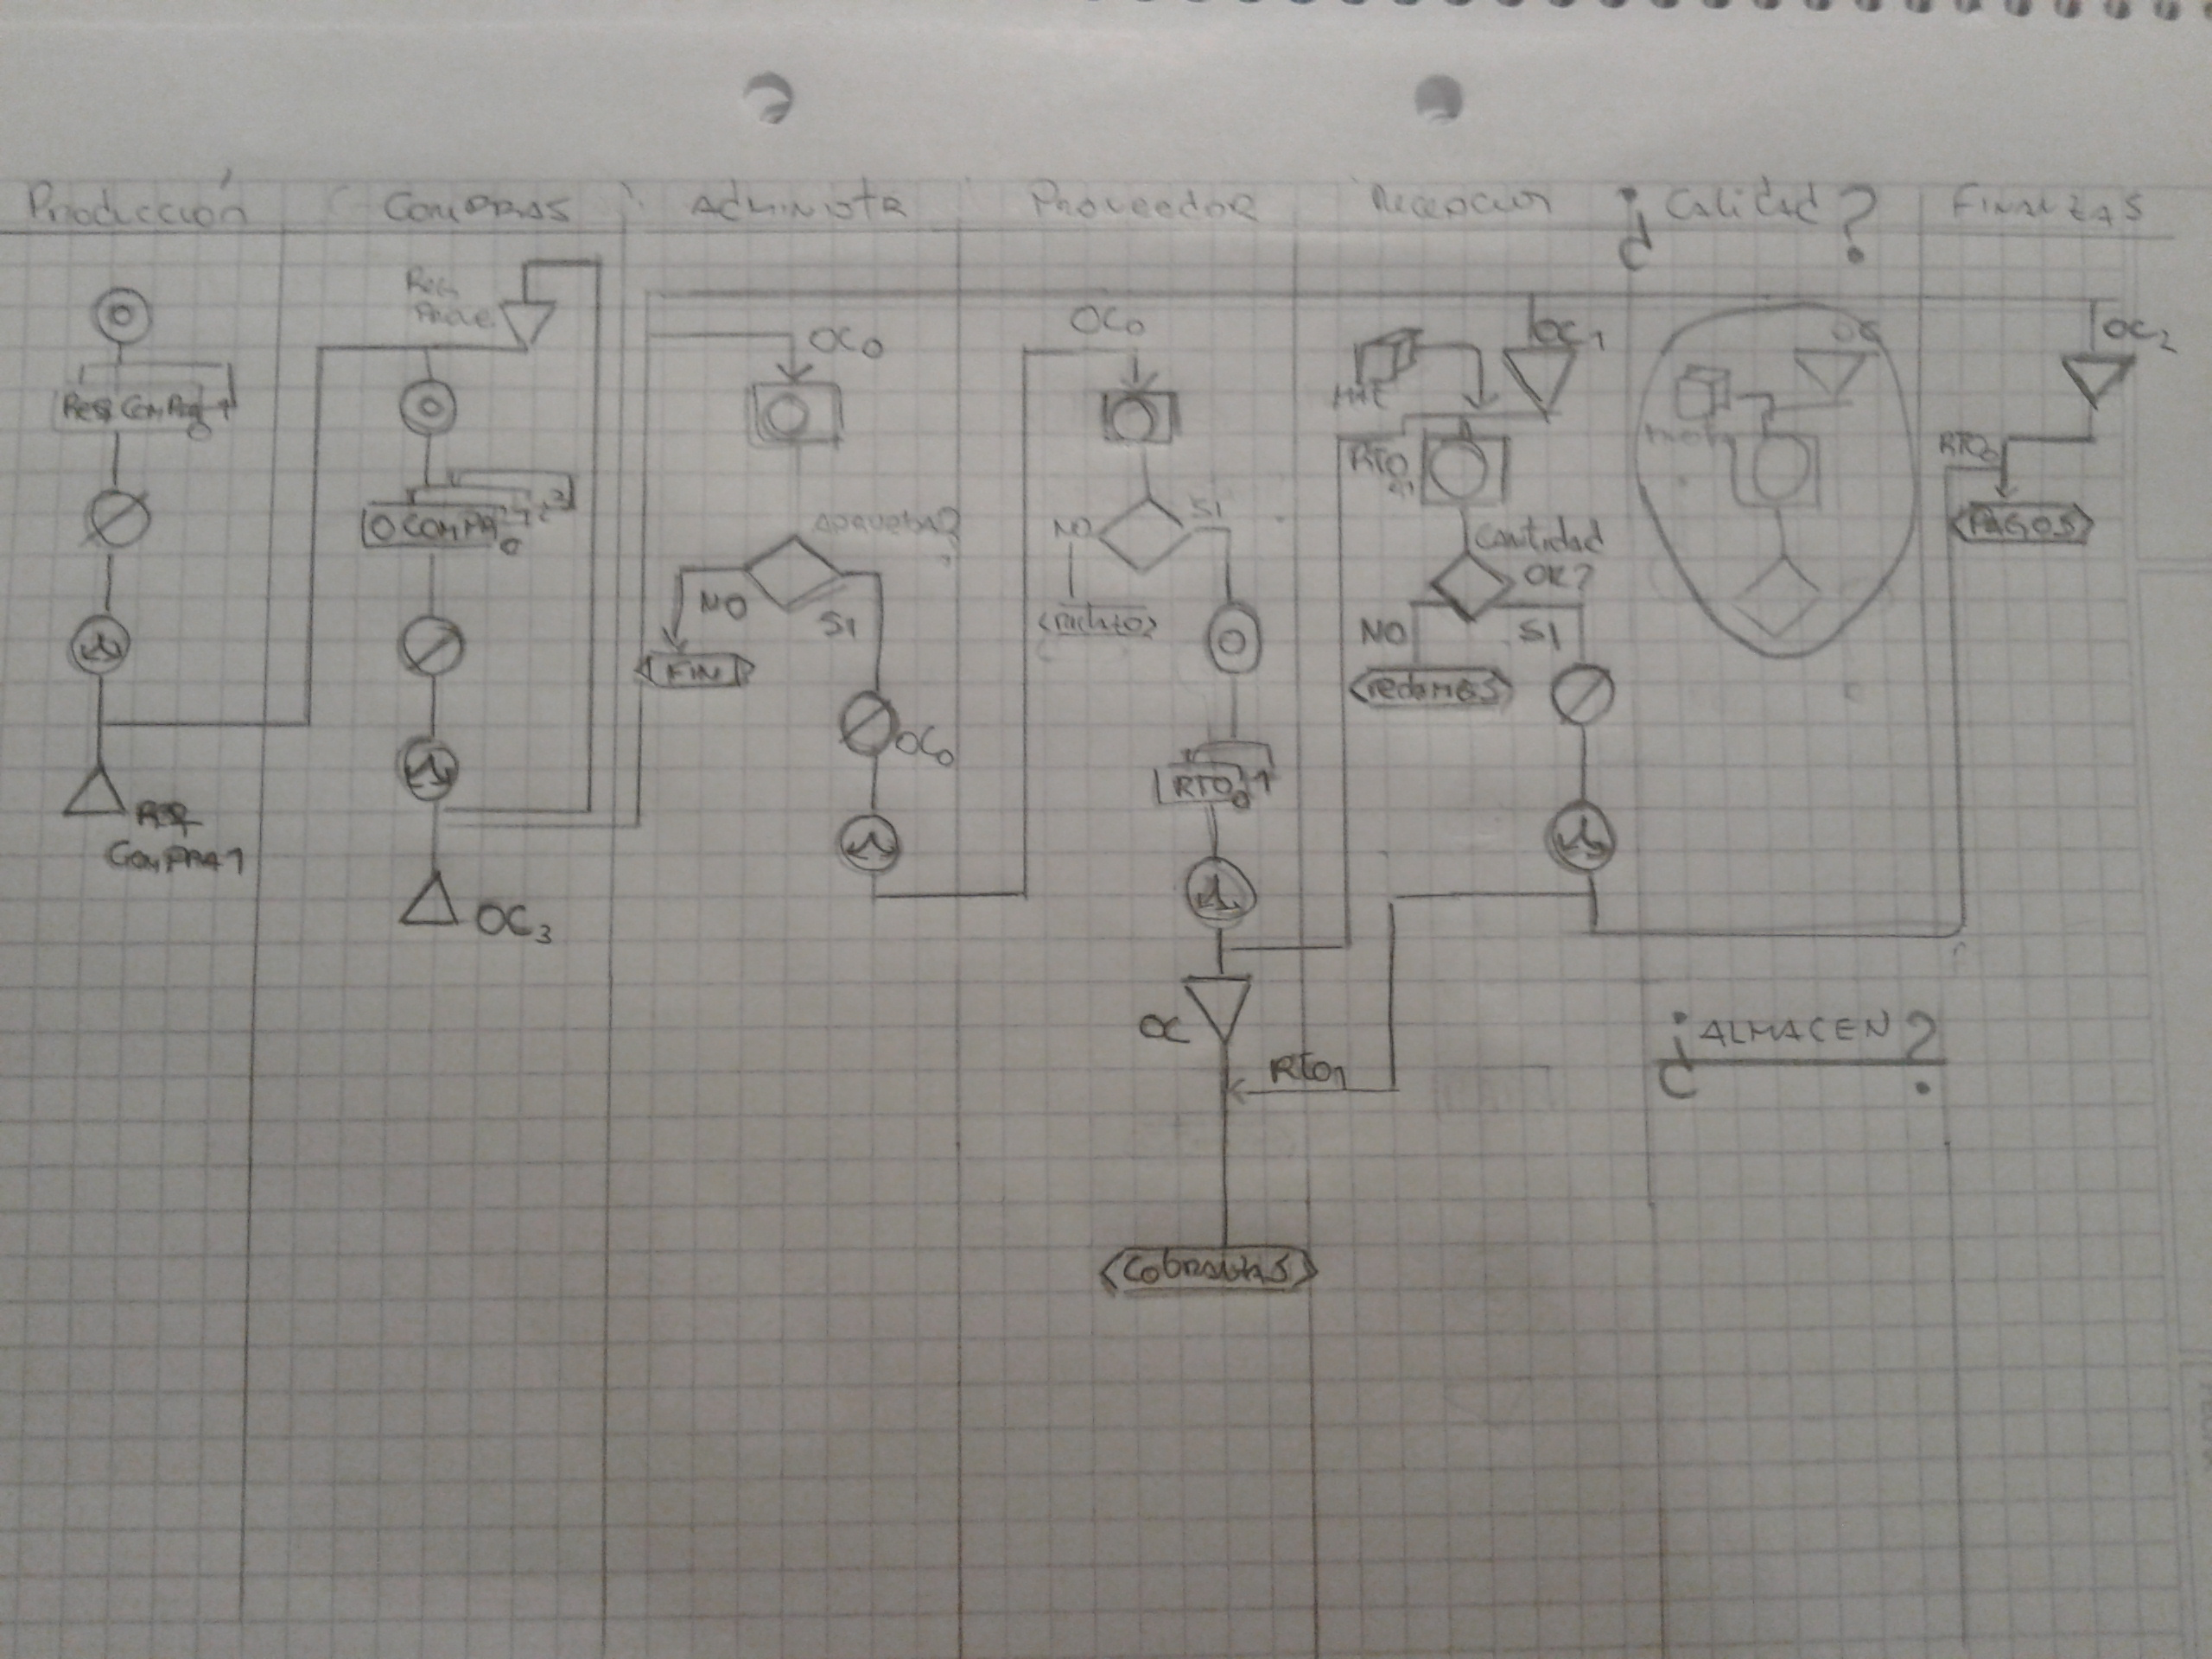
\includegraphics [angle=90,width=\linewidth]{Empresa/Circuitos/Compras/Compras.jpg}

\pagebreak

\subsubsection{Procedimiento}
\begin{description}
\item[Producción] Tras detectar necesidad de materiales y luego de chequear las existencias, el sector de Producción emite el documento Requerimiento de Compra (RC), lo firma el nivel autorizante y lo envía al sector de Compras.
\item[Compras] Recibido el Requerimiento de Compra, el área de Compras consulta catálogos y listas de precios de los proveedores, y en función de ellos confecciona una Orden de Compra (OC) original y tres copias, las firma y distribuye original a Dirección General y dos duplicados, uno a recepción, y otro a finanzas, y almacena una copia.
\item [Dirección General] Tras recibir la Orden de Compra del sector de Compras, la Dirección General la controla, y en caso de aprobarla la firma y envía al sector de Ventas del Proveedor previamente seleccionado
\item [Proveedor] Una vez recibida la Orden de Compra firmada por Compras y Dirección General el Proveedor rechaza la Orden de Compra o la aprueba. En caso de aprobación, el proveedor confecciona Remito por duplicado y envía original y una copia junto con los materiales al sector de Recepción.
\item[Recepción] Tras recibir los materiales y el Remito original y una copia, el sector de Recepción controla cotejando cantidades en ambos contra la Orden de Compra. En caso de concordar, ingresa la mercadería en su almacén y firma Remito original y copia, distribuye el original al sector Finanzas y la copia al Proveedor.
\item[Finanzas] Una vez recibido el remito del Proveedor se controla contra la Orden de Compra y se procede a continuar al circuito no relevado de Pagos.
\item [Proveedor] Recibido el remito firmado se continua con el Circuito no relevado de Cobranzas.
\end{description}